\section{Mapping rules in spreadsheets: Mapeathor}
\label{sec:chp5_mapeathor}

Ever since the adoption of mapping languages increased, multiple  editors were developed to ease the mapping writing proces and assist the needs of the user. Some of the developed approaches enable editing through graphical visualization~\citep{heyvaert2016rmleditor,sicilia2017map}, while others provide a writing environment (e.g. Ontop for Protégé\footnote{\url{https://ontop-vkg.org/tutorial/basic/setup.html\#ontop-protege-setup}}). Yet, these editors are language-oriented, as they help to create mappings in a specific language. In real world scenarios, however, different use cases require different features and implementations. As a result, several different mapping languages are used currently, while the interoperability among them is very limited~\cite{iglesias2022devising}. Moreover, graphical interfaces can result cumbersome as the number of mapping rules increase, becoming inconvenient for high-demanding use cases. 

%Moreover, when managing large amounts of mapping rules, graphical interfaces become cumbersome. %With our approach we aim at easing the writing process using a common tool such as spreadsheets, as well as enabling the generation of mapping files in more than one mapping language.

%In our work we focus on facilitating the transformation rule specification using declarative mapping rules. 
This section presents a straightforward approach to generate mapping documents leveraging the specification of mapping rules in spreadsheets. These spreadsheets contain the essential elements of the mapping rules without any additional syntax element, and are later translated into one a mapping document. The purpose of this approach is to ease the mapping writing process for practitioners, as well as to increase the interoperability among them~\citep{corcho2020towards, iglesias2022devising}. This approach is implemented in Mapeathor~\citep{iglesias-molina_2023_5973906}, a tool able to parse the spreadsheets and generate the corresponding mappings in R2RML, RML and YARRRML. Following, we present the structure of the spreadsheet to write the mapping rules, the implementation and a evaluation with a user study to analyse the fitness of our approach.

\subsection{Spreadsheet-based Mapping Rules}
\label{sec:chp5_spreadsheet_design}

%The rules required to generate a knowledge graph can be specified in multiple languages. The language is chosen by the user depending on the specific use case. However, the rules themselves are equivalent across languages, so they can be written in a language-independent way, in this case, we chose a spreadsheet for rule specification. 

This section presents the design of the spreadsheet template to write the mapping rules. 
These mapping rules are written following template that contains only the essential information to later generate the mapping. 
This design is devised to represent the rules in a compact and understandable manner, using a format widely used by the scientific community (i.e. Google spreadsheets, MS Excel).
Thus, this approach prevents the user from learning the particular syntax of each language (e.g. keywords, semicolons, brackets, etc.) while using a familiar environment for writing the spreadsheets. 

The spreadsheet template consists of five different sheets, which are described below: \textit{Prefix sheet}, \textit{Source sheet}, \textit{Subject sheet}, \textit{Predicate\_Object sheet} and \textit{Function sheet}. We illustrate this section with a running example to describe in detail the expressiveness capabilities of each spreadsheet. This example uses the data represented in the CSV file \texttt{people.csv}(\cref{lst:chp5-1_mapeathor_input_people}) and the JSON file \texttt{sport.json} (\cref{lst:chp5-1_mapeathor_input_sport}).

\begin{minipage}{0.48\linewidth}
\begin{captionedlisting}{lst:chp5-1_mapeathor_input_people}{ Contents of \texttt{people.csv}.}
\centering
\begin{tabular}{c}
%\hspace{1em}
{
\begin{lstlisting}[basicstyle=\ttfamily\small,label={list:example1},columns=flexible]
id , name  , birthdate , sport_id
1  , Emily , 08/02/90  , 2
2  , Jonah , 18/11/75  , 2
\end{lstlisting}
}
\end{tabular}
\end{captionedlisting}
\end{minipage}
\,\,\,\,\hfill
\begin{minipage}{0.52\linewidth}
\begin{captionedlisting}{lst:chp5-1_mapeathor_input_sport}{Contents of \texttt{sport.csv}.}
\centering
\begin{tabular}{c}
\hspace{1.5em}
{
\begin{lstlisting}[basicstyle=\ttfamily\small,label={list:example1},columns=flexible]
[ {
   "id": 1,
   "sport": " Ice Skating"
 },{
   "id": 2,
   "sport": " Rugby"
 } ]
\end{lstlisting}
}
\end{tabular}
\end{captionedlisting}
\end{minipage}


\subsubsection{Prefix sheet} 
This sheet contains the namespaces and corresponding prefixes used in the creation of the transformation rules. 
It is composed of two columns: \texttt{Prefix} for the prefix and \texttt{URI} for the corresponding namespace. The base namespace can be specified writing ``@base" in the \texttt{Prefix} column. 
The example shown in \cref{tab:chp5-1_prefix_sheet} presents how three namespaces and the base namespace are written in this template. 

\begin{table}[h!]
\caption{Prefix sheet.}
\label{tab:chp5-1_prefix_sheet}
\centering
\begin{tabular}{c|c}
\midrule
\textbf{Prefix} & \textbf{URI}                                 \\ \midrule
@base           & http://example.com/                          \\
rdf             & http://www.w3.org/1999/02/22-rdf-syntax-ns\# \\
ex              & http://ex.com/                               \\ 
grel            & http://semweb.datasciencelab.be/ns/grel\#     \\
\midrule
\end{tabular}
\end{table}


\subsubsection{Subject sheet} 
This sheet defines how to generate the subjects and a corresponding identifier (\texttt{ID}) that groups the mapping rules per subject. It is organized in four columns: \texttt{ID}, \texttt{URI}, \texttt{Class} and \texttt{Graph}. \texttt{ID} contains a unique identifier for each subject's set of rules in order to relate to information on these rules in the remaining sheets.
\texttt{URI} defines the subject URI of the resources that are to be generated by the mapping. 
\texttt{Class} allows the assignation of the subject to a class with \texttt{rdf:type}. A subject may be type of one class, more than one or none at all. 
Finally, \texttt{Graph} is an optional column that enables the assignation of a named graph to the triples generated for a subject.

The example shown in \cref{tab:chp5-1_subject_sheet} presents how to write two subjects, each with a different identifier and URI for the instances. Within the \texttt{URI} field, what is written between ``\{" and ``\}" references a field in the source data. The instances of the subject with the \texttt{PERSON} ID are type of two classes, (\texttt{ex:Person} and \texttt{ex:Athlete}), while all the triples of the instances of the subject identified with the \texttt{SPORT} ID are assigned to a named graph (\texttt{ex:SportsGraph}). 


\begin{table}[h!]
\caption{Subject sheet.}
\label{tab:chp5-1_subject_sheet}
\centering
\begin{tabular}{c|c|c|c}
\midrule
\textbf{ID} & \textbf{URI} & \textbf{Class} & \textbf{Graph} \\ \midrule
PERSON & http://ex.com/Person/\{name\} & ex:Person &  \\
PERSON & http://ex.com/Person/\{name\} & ex:Athlete &  \\
SPORT & http://ex.com/Sport/\{sport\} & ex:Sport & ex:SportsGraph \\ \midrule
\end{tabular}
\end{table}



\subsubsection{Source sheet} 

This sheet describes the source input data for each set of rules, identified with the identifier previously created in the \textit{Subject sheet} (\texttt{ID}). The information is organized in three columns: \texttt{ID}, \texttt{Feature} and \texttt{Value}. 
\texttt{ID} makes reference to the identifier that gathers the mapping rules in the sheets (introduced in the \textit{Subject sheet}). 
\texttt{Feature} declares the type of information provided in \texttt{Value}. The allowed keywords in this column are: \texttt{source} for the path and name of the file, \texttt{format} for the data source format, \texttt{iterator} for hierarchical data (e.g. JSON, XML), \texttt{table} for name of tables from Relational Data Bases (RDBs), \texttt{query} for SQL queries and \texttt{SQLVersion} for the version of SQL used. Each ID must have at least the \texttt{source} and \texttt{format} features specified, the rest of the features are optional. 
Then, in the \texttt{Value} column, the corresponding values of each \texttt{Feature} specified are written. 

\cref{tab:chp5-1_source_sheet} shows the data source description for the \texttt{PERSON} and \texttt{SPORT} IDs. The former describes as input data the CSV file shown in \cref{lst:chp5-1_mapeathor_input_people}, while the latter describes the JSON file in \cref{lst:chp5-1_mapeathor_input_sport}, for which the iterator is also written (\texttt{\$.*}). 

\begin{table}[h!]
\caption{Source sheet.}
\label{tab:chp5-1_source_sheet}
\centering
\begin{tabular}{c|c|c}
\midrule
\textbf{ID} & \textbf{Feature} & \textbf{Value}              \\ \midrule
PERSON    & source          & /home/user/data/people.csv  \\
PERSON    & format          & CSV                         \\
SPORT     & source          & /home/user/data/sports.json \\
SPORT     & format          & JSON                        \\  
SPORT     & iterator        & \$.*                    \\ \midrule
\end{tabular}
\end{table}

\subsubsection{Predicate\_Object sheet} 
This sheet enable users to specify how to generate the triples, that is, predicate-object pairs for the subjects defined in the \textit{Subject sheet}. This sheet contains up to 8 columns: \texttt{ID}, \texttt{Predicate}, \texttt{Object}, \texttt{DataType}, \texttt{Language}, \texttt{ReferenceID}, \texttt{InnerRef} and \texttt{OuterRef}.

The column \texttt{ID} indicates the set of rules which the triples belong to, that has been previously defined in the \textit{Subject} and \textit{Source sheets}.
The columns \texttt{Predicate} and \texttt{Object} specify the predicate and object of the triple respectively. 
The XSD datatype of \texttt{Object} is defined in \texttt{DataType}, and the language tag in \texttt{Language}. Both these columns are optional. 

When the object refers to a subject defined in another mapping rule, the rule is written as follows. 
There are three columns that allow the specification of the linking condition between the object of the current triple and the referenced subject. 
They specify which is the ID of the referred subject  (\texttt{ReferenceID}), and the ``join'' fields in the source data: (i) \texttt{InnerRef} for the field of the object of the current triple, and (ii) \texttt{OuterRef} for the field of the referred subject. These three fields can be blank when a regular triple is produced. 

\cref{tab:chp5-1_po_sheet} shows five predicate-object pairs created for both sets of rules (\texttt{PERSON} and \texttt{SPORT}. Three of these rules produce literals with datatypes and two additionally specify a language tag. The rule set identified as \texttt{PERSON} generates a link to the subject of the \texttt{SPORT} rule set using the predicate \texttt{ex:name}, and joining by equal values of the field \texttt{sport\_id} from \texttt{people.csv} and the field \texttt{id} from \texttt{sport.json}. This rule set also calls a function for generating the object for the predicate \texttt{ex:birthdate}, which is identified by being enclosed by ``$<>$".

\begin{table}[h!]
\caption{Predicate\_Object sheet.}
\label{tab:chp5-1_po_sheet}
\centering
\resizebox{\columnwidth}{!}{
\begin{tabular}{c|c|c|c|c|c|c|c}
\midrule
\textbf{ID} &\textbf{Predicate} & \textbf{Object}               & \textbf{DataType} & \textbf{Language} & \textbf{ReferenceID} & \textbf{InnerRef} & \textbf{OuterRef} \\ \midrule
PERSON & ex:name & \{name\} & string & en & & &  \\
PERSON & ex:birthdate & $<$Fun-date$>$ & & & & & \\
PERSON & ex:plays & & & & SPORT& sport\_id & id \\
SPORT & ex:name & \{sport\} & string & en & & & \\
SPORT & ex:code & \{id\} & integer & & & & \\ \midrule
\end{tabular}
}
\end{table}

\subsubsection{Function sheet} Some languages are able to process data transformation functions, which can be detailed in this sheet. Mapeathor implements the last release of the RML-FNML specification, that describes how to incorporate functions in RML mappings\footnote{\url{https://w3id.org/rml/fnml/spec}}. The functions are referred in the \textit{Predicate\_Object sheet} or in other function rows with the identifier specified in \texttt{FunctionID}. The column \texttt{Feature} is used to specify the type of information provided in \texttt{Value}. The features admitted in the \texttt{Feature} column are \texttt{executes} for the name of the function, and \texttt{returns} for the expected output type of the function. In addition, this column admits any number of function parameter names. Then, the value of the name of the function, return type and values of the parameters are written correspondingly in the \texttt{Value} column.

The example shown in \cref{tab:chp5-1_function_sheet} uses the function \texttt{grel:toDate}, to change the formatting of a date. It returns a date as output (\texttt{grel:dateOut}) and takes three parameters: the data field to be converted (\texttt{grel:valueParam1}), the input data format (\texttt{grel:valueParam2}) and the output data format (\texttt{grel:valueParam3}).

\begin{table}[h!]
\caption{Function sheet.}
\label{tab:chp5-1_function_sheet}
\centering
\begin{tabular}{c|c|c}
\midrule
\textbf{FunctionID} & \textbf{Feature} & \textbf{Value} \\ \midrule
$<$Fun-date$>$ & executes & grel:toDate \\  
$<$Fun-date$>$ & returns & grel:dateOut \\  
$<$Fun-date$>$ & grel:valueParam1 & \{birthdate\} \\
$<$Fun-date$>$ & grel:valueParam2 & dd/MM/yyyy \\
$<$Fun-date$>$ & grel:valueParam3 & yyyy-MM-dd \\
\midrule
\end{tabular}
\end{table}


\subsection{Implementation: Mapeathor}
\label{sec:chp5_mapeathor_tool}

Mapeathor~\citep{iglesias-molina_2023_5973906} is a open-source implementation to generate mappings from the spreadsheets described in \cref{sec:chp5_spreadsheet_design}. It is able to process MS Excel and Google Spreadsheets, generating human-readable mappings in either R2RML, RML or YARRRML. 

\cref{alg:mapeathor} presents the procedure implemented by Mapeathor to translate an input spreadsheet into a formatted mapping document. First, the rules written in the spreadsheet template are extracted and stored in a JSON file. This step also validates that the spreadsheet follows correctly the template. The prefixes are then added to the output mapping document, along with other prefixes that are used nativetly in the target language (e.g. \texttt{rr}\footnote{\url{http://www.w3.org/ns/r2rml\#}}, \texttt{rml}\footnote{\url{http://semweb.mmlab.be/ns/rml\#}} \ana{prefijo rml}). Then, the rules are translated by grouping them into rulesets with the same \texttt{ID} expressed in the spreadsheet (see \cref{sec:chp5_spreadsheet_design}). The extracted rules are enriched with implicit information needed to write the mapping (e.g. to look for \texttt{rr:TermTypes} and IRIs). Next, the subject, source and predicate-object pairs in each ruleset are translated. In the case of RML, the system also looks for referencing functions to translate them as well. Finally, the translated rules are written into a final file, which is returned as output. 



The mapping documents are generated in a human-readable manner considering previous experiences~\citep{chaves2022systematic,corcho2021high,chaves2020bench}.
This helps knowledge engineers in complex data integration contexts to understand more easily if the mapping document represents the desirable rules originally written and, hence, whether the constructed knowledge graph will be correct or not. 
For [R2]RML, the output mapping follows a Turtle-based syntax, using predicate object lists within blank node properties\footnote{\url{https://www.w3.org/TR/turtle/\#unlabeled-bnodes}}, as recommended by the [R2]RML specifications.
We also ensure the same mapping rules' order as they are defined in the spreadsheet.
\cref{sec:appendix-mapeathor} shows the output mappings produced by Mapeathor after processing the rules written in the spreadsheet shown in Tables \ref{tab:chp5-1_prefix_sheet}, \ref{tab:chp5-1_subject_sheet}, \ref{tab:chp5-1_source_sheet}, \ref{tab:chp5-1_po_sheet} and \ref{tab:chp5-1_function_sheet}, also available online\footnote{\url{https://docs.google.com/spreadsheets/d/1sJ_LM3AJlIopFDJx8GC_afoM0MX583GVt-clVJ2oOOs/}}


\begin{minipage}{0.95\linewidth}
\begin{algorithm}[H]
\SetAlgoLined
\KwResult{Mapping document in [R2]RML/YARRRML}
 $language \longleftarrow output\_language$\;
 $spreadsheet \longleftarrow input\_spreadsheet$\;
 $output\_m \longleftarrow \emptyset$\;
 $rules \longleftarrow extract\_rules(spreadsheet)$\;
 $output\_m.add(translate\_prefixes(rules))$\;
  
 \For{$ruleset \in rules$}{
    $rules.add(enrich\_ruleset(ruleset))$\;
    $output\_m.add(translate\_subject, language)$\;
    $output\_m.add(translate\_source, language)$\;
    $output\_m.add(translate\_predicate\_object, language)$\;
    \If{$language == RML$}{
        $output\_m.add(translate\_functions)$\;
        }
    }
 
 \Return{$validate(write\_m)$}\;
\caption{Mapeathor translation algorithm}
\label{alg:mapeathor}
\end{algorithm}
\end{minipage}


The source code of Mapeathor is openly available under Apache 2.0 license\footnote{\url{https://github.com/oeg-upm/mapeathor}}. It can be run as a CLI using the Pypi package\footnote{\url{https://pypi.org/project/mapeathor/}} or as an online service\footnote{\url{https://morph.oeg.fi.upm.es/demo/mapeathor}}, where a visual interface is provided. With each release, a new version in Pypi is created and a dedicated DOI archived in Zenodo~\citep{iglesias-molina_2023_5973906}. 




\subsection{Evaluation}
We evaluate the presented approach by performing a user study to test %the usability of Mapeathor and check 
if the spreadsheet-based approach can improve the mapping writing process for users of different expertise. 

%\begin{table}[t!]
%\caption[]{Questionnaire for subjective assessment of the usability of the spreadsheet design and Mapeathor. }
%\centering
%\label{tab:chp5-1_sub_questionnaire}
%\resizebox{\columnwidth}{!}
%{\begin{tabular}{cl}
%\multicolumn{2}{c}{\textbf{Questions}} \\ \midrule
%1. & I think that I would like to use this tool frequently\\ \midrule
%2. & I found the tool unnecessarily complex\\ \midrule
%3. & I thought the spreadsheet template was easy to use\\ \midrule
%4. & I think that I would need the support of a technical person to be able to use the spreadsheet template\\ \midrule
%5. & I found the different facets in this spreadsheet template were well integrated\\ \midrule
%6. & I thought there was too much inconsistency in this tool\\ \midrule
%7. & I think that most people would learn how to write the spreadsheet template very quickly\\ \midrule
%8. & I found the tool unmanageable to use\\ \midrule
%9. & I felt very confident using the spreadsheet template\\ \midrule
%10. & I needed to learn a lot of things before I could get going with this tool\\ \midrule
%11. & Optional comments (feedback to improve) \\ \bottomrule
%\end{tabular}}
%\end{table}

\subsubsection{Methodology}
\label{sec:chp5_mapeathor_eval_method}

%The evaluation is performed in two steps. We first carry out a \textit{subjective evaluation} in order to gather opinions and feedback about the spreadsheet template and usability of the tool in order to improve the user experience. We then perform a \textit{objective evaluation} 
The evaluation performed consist of a user study that aims at
testing if our approach improves the mapping writing process w.r.t. writing directly the mapping in a target language (i.e. RML) and w.r.t. another mapping editor with a visual interface (i.e. RMLEditor). This section describes the methodology followed.

%\textit{motivación: qué queremos comprobar, que si facilita la creación de mapping rules para experts y no experts. Para eso llevamos a cabo dos evaluaciones con usuarios, subjectiva y objetiva. En la subjectiva usuarios que han probado el software cuentan su experiencia y opiniones. En la objetiva, cogemos a usuarios y los dividimos en 3 grupos, para que generen mappings con rml, rmleditor y mapeathor. Así vemos si 1) mapeathor mejora RML y si 2) funciona mejor que una herramienta visual. Describir background, que no hay bias porque se puso a gente que nos había utilizado esa tech antes. y resultados}


\noindent\textit{\textbf{Procedure}} 
%The evaluation is comprised of two steps. The first step, correspondent to the \textit{subjective evaluation}, took place during the Knowledge Graph Construction Tutorial co-located with the 19th edition of the Extended Semantic Web Conference (2022)\footnote{\url{https://kg-construct.github.io/eswc-dkg-tutorial-2022/}}. This tutorial hosted a slot for presenting Mapeathor and the spreadsheet design, allowing time for a hands-on exercise at the end of the explanation. At the end of the slot, participants were asked to fill a questionnaire to assess the usability of the approach and gather some feedback for improvements. The questionnaire first inquired about the background of the participants, asking them to rate in a 5-point Likert scale their expertise in (i) linked data and (ii) mapping languages and tools. Then, it assessed the usability of the approach with 10 questions that follow the SUS template, with also a 5-point Likert scale rating; and an additional optional question to gather feedback for improvement (\cref{tab:chp5-1_sub_questionnaire}).
%The second step of the evaluation that comprises the \textit{objective evaluation} 
The user study took place in May 2023. %, once the improvements gathered from the previous step were implemented. 
In this step, the spreadsheet-based approach proposed in this work was compared with the widely used RML mapping language~\citep{Dimou2014rml}, and with a visual editor, RMLEditor~\citep{heyvaert2016rmleditor}. A group of 30 participants was divided into three groups of 10. Each group had to carry out the same task, to create a mapping from a given dataset and ontology with the assigned tool. All groups were introduced to the needed concepts about mapping languages and specific guidelines with examples of the assigned tool. The groups performed the given task in separated sessions, i.e. one session per tool was carried out, to ensure that all participants were given the same level of assistance independently of the tool. Participants were asked to carry out the proposed task in 30 minutes. Having reached the time limit, they were asked to submit the mapping written so far. In addition, participants were asked to rate in a 5-point Likert scale their expertise in (i) linked data and (ii) mapping languages and tools; and to write their personal opinion on the assigned tool.


\begin{figure*}[!t]
\centering
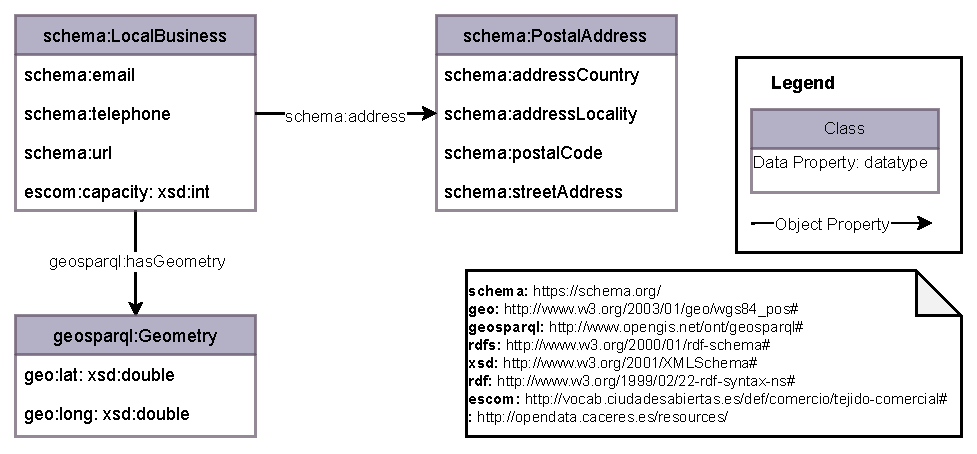
\includegraphics[width=\linewidth]{figures/chp5-1_us_onto.pdf}
\caption[Ontology diagram for the user study exercise of Mapeathor]{Ontology diagram representing a subset of the Vocabulary for data representation of the local business census and activities licenses.}
\label{fig:chp5-1_us_onto}
\end{figure*}

\noindent\textit{\textbf{Resources}}
The same data and ontology was used for both evaluations. We use a subset of the \textit{Vocabulary for data representation of the local business census and activities licenses}\footnote{\url{http://vocab.ciudadesabiertas.es/def/comercio/tejido-comercial/index-en.html}} that represents local businesses, their postal address and geolocalization (\cref{fig:chp5-1_us_onto}). 
We chose this dataset, that belongs to the common-knowledge domain, to avoid heterogeneous prior domain knowledge influence on the results of the study.

We provided participants with the subset ontology description and associated data, that is comprised of three CSV files: \texttt{bar.csv}, \texttt{restaurant.csv} and \texttt{address.csv}. Information about bars, restaurants and their geolocalization is represented in the files \texttt{bar.csv}, \texttt{restaurant.csv} respectively. 
These files contain the same columns, but different data. The file \texttt{address.csv} represent the postal address of the businesses present in the other two files. 
The original data is available in GitHub\footnote{\url{https://github.com/CiudadesAbiertas/vocab-comercio-censo-locales/}}. 
To facilitate the exercise for participants, some data cleaning was performed over the original files, as well as translation to all columns form spanish to english. The used resources are published in Zenodo~\citep{iglesias-molina_2022_8154522}.



\noindent\textit{\textbf{Participants}} 
%In the \textit{subjective evaluation}, 17 attendants submitted answers to the questionnaire provided during the session. Most of the participants were knowledgeable in linked data, while less than half had already used mappings before. 
%In the \textit{objective evaluation}, 
There were in total 30 participants, all sampled from the Ontology Engineering Group, ranging from MSc students to full professors. Their background ranged from having basic knowledge about linked data and mappings, to being knowledgeable practitioners, including participants that were experts in linked data but had no knowledge about mappings. Prior to the assignation of participants to each group, participants were asked to provide information about whether they had prior knowledge of any of the tools, so that no participant would use a tool which they were already familiar with. Taking into account this restriction, they were randomly divided into three groups, one per tool. Each group was balanced w.r.t. the heterogeneity in background (\cref{fig:chp5-1_expertise}). 


\begin{figure*}[!t]
\centering
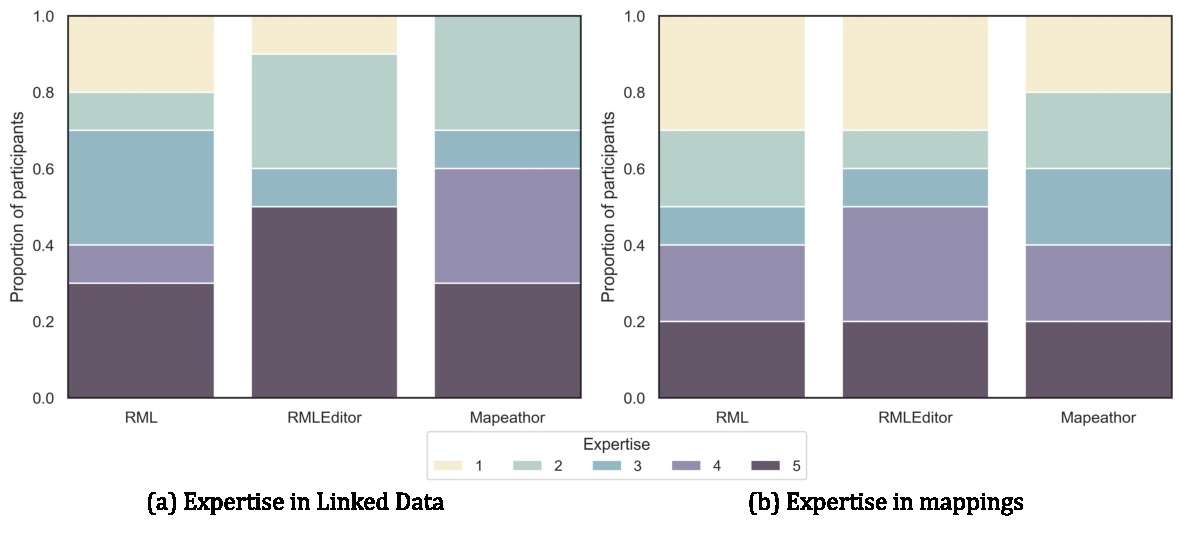
\includegraphics[width=1\linewidth]{figures/chp5-1_expertise.pdf}
\caption[Expertise of participants of the user study]{Distribution of expertise of participants according to the 5-point Likert scale in (a) Linked Data and (b) mappings.}
\label{fig:chp5-1_expertise}
\end{figure*}

\noindent\textit{\textbf{Metrics}} 
%The \textit{subjective evaluation} measured the responses to the SUS questionnaire on a 5-point Likert scale. 
%For the \textit{objective evaluation},
We calculate two kinds of measurements for accuracy: (i)~\textit{Total Accuracy} (TA) for the number of correct rules written w.r.t. the reference correct mapping, and (ii)~\textit{Local Accuracy} (LA) for the number of correct rules w.r.t. all the written rules. We calculate both accuracies because of the fixed time for completing the exercise. TA can be interpreted as a measure of completeness, while LA focusses on assessing the correctness of the written rules independently on the total completeness.
We divide the mapping in four components: \textit{Subject}, \textit{Source}, \textit{Predicate-Object (PO)} and \textit{Join}, and calculate the accuracy for each component and the totality of the mapping. Then a T-Test is performed to look for significant differences of accuracy among the tools. This test is sed under the assumptions of (i) normality, (ii) sameness of variance, (iii) data independence, and (iv) variable continuity.


\noindent\textit{\textbf{Threats to validity}}~\citep{creswell2017research} We identify the following internal and external threats to the validity of our experiment.

\textbf{Internal validity threats} concern the experimental setup or experience of participants which threaten the ability to draw correct conclusions about the population in the experiment. We identify three internal threats: \textit{tool familiarity bias}, \textit{selection bias} and \textit{instruction bias}.
\begin{itemize}
    \item \textbf{Tool familiarity bias.} Practitioners tend to be more expert in some specific technologies and languages that they use more frequently. Thus, in the sample there it is possible to have participants that have used any of the tested approaches, which in turn can influence the results. For creating the groups, participants' experience was inquired to avoid assigning them a tool that they had previously used.
    \item \textbf{Selection bias.} The sample includes participants with different range of skills and previous knowledge about linked data and mappings. We mitigate this threat by defining groups that were  homogeneous w.r.t. range of expertise in mappings and linked data, considering also the mitigation measures for the \textit{tool familiarity} threat. That is to say, all groups included from beginner users to knowledgeable practitioners. 
    \item \textbf{Instruction bias.} One of the evaluated approaches is designed by the conductors of the user study. This situation could incur in bias on information delivery. To mitigate this threat, we provided participants with the same instruction guidelines for each tool. Three sessions were conducted subsequently to provide the same explanations and attention to each tool. During each sessions, all questions were answered with equal level of detail and guidance for all tools and participants.
\end{itemize}

\textbf{External validity threats} occur when wrong inferences from sample data are made beyond the studied sample or experimental setup. We identify two external threats: \textit{background of participants sample} and \textit{environment}.
\begin{itemize}
    \item \textbf{Background of participants sample.} This threat concerns the generalization to individuals outside the study. The sample of participants include a wide range in the variety of backgrounds, from not very familiar with linked data and mappings, to expert practitioners. We deliberately choose to have this variety for each group so that the results can be generalized to a broader sample, while mitigating the risks of internal threats described above that this choice poses. 
    \item \textbf{Environment.} This threat concerns the generalization to individuals outside the experiment’s setting. Participants were free to use a computer, browser and tools of their choice. Thus, they could perform the tasks required for the study in a well-known environment. No specific experimental setup prevents generalizations to individuals outside our study.
\end{itemize}




\subsubsection{Results}
\label{sec:chp5_mapeathor_results}

%\noindent\textit{\textbf{Subjective evaluation results}}


\begin{figure}[t!]
    \centering
    \begin{subfigure}[b]{\linewidth}
    	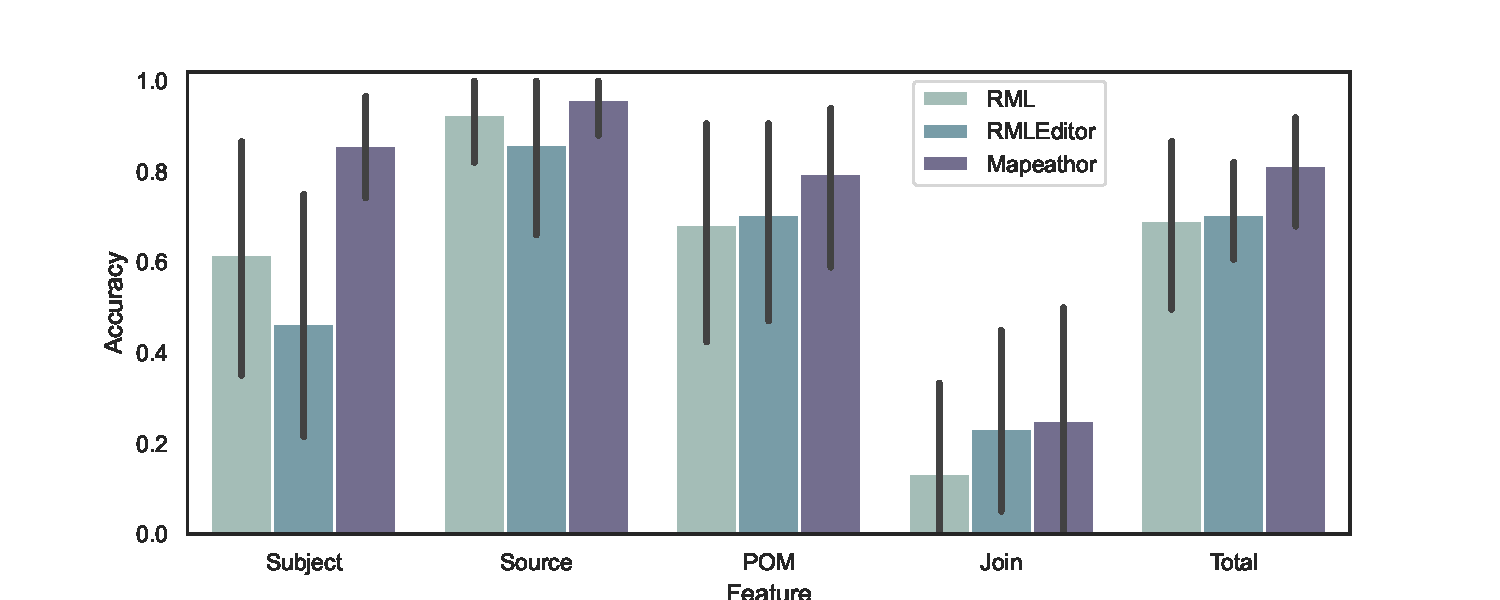
\includegraphics[width=\linewidth]{figures/chp5-1_rel-acc.pdf}
    	\caption{Local accuracy.}
    	\label{fig:chp5_mapeathor_relacc}
    \end{subfigure}
   %\hspace{0.05\textwidth}
    \begin{subfigure}[b]{\linewidth}
    	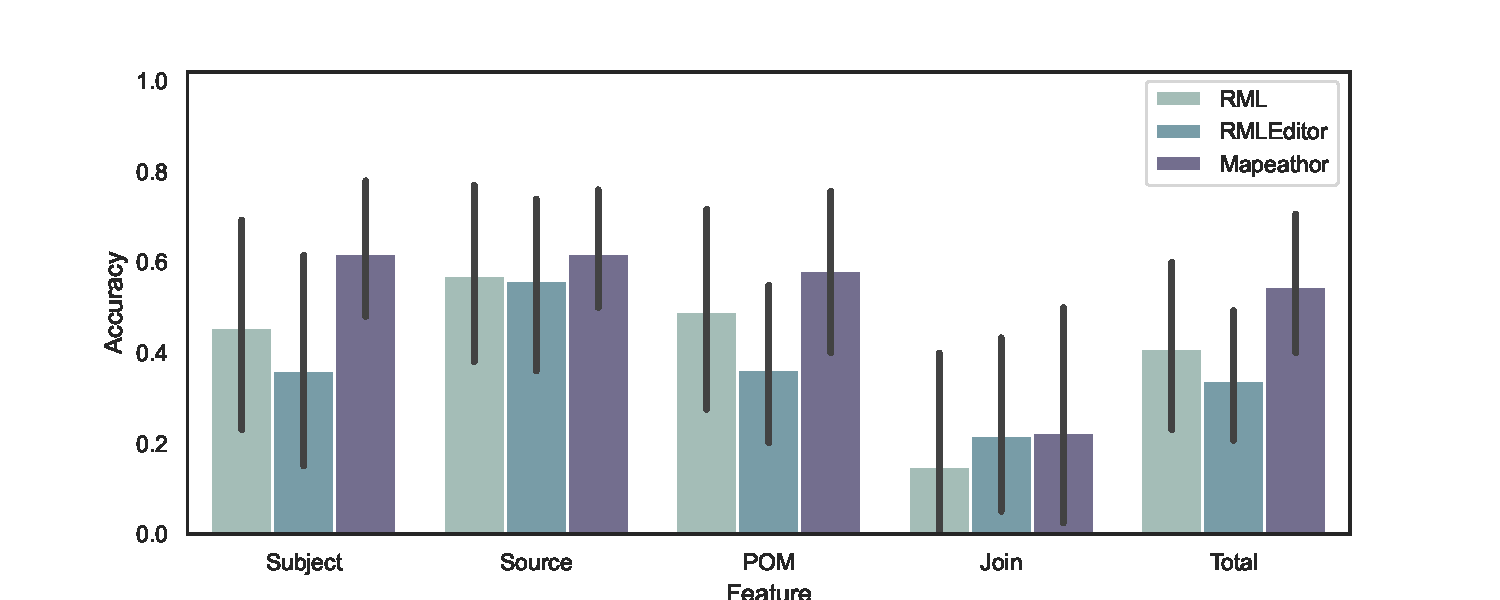
\includegraphics[width=\linewidth]{figures/chp5-1_total-acc.pdf}
    	\caption{Total accuracy.}
    	\label{fig:chp5_mapeathor_totacc}
    \end{subfigure}
    \caption[Accuracy results of user study]{Local accuracy (a) and Total accuracy (b) of the mappings written by participants of the user study.}
    \label{fig:chp5-1_accuracy}
\end{figure}

%\noindent\textit{\textbf{Objective evaluation results}}

%\ana{e ir intercalando opiniones sobre cada approach para apoyar los resultados, ambas buenas y malas}
%\ana{de rmleditor fallos a nivel técnicos, opiniones divididas entre intuitivo/antiintuitivo, hay constructos que hay que explicar, pero una vez superada esa barrera medianamente bien. Remarcan que faltan funcionalidades como copy/paste de secciones enteras, y buscar mejor lo creado en el espacio de trabajo (a muchos se les perdían las cosas y había que volver a empezar)}
%\ana{de rml igual hay mejores resultados porque una vez se entienden las partes del mapping y partiendo de un ejemplo, qué hay que copiar y cambiar, eso agiliza el proceso. Más indicado para desarrolladores (más acostumbrados a escribir código), se señala que no es excesivamente complejo pero con alguna herramienta se haría mejor.}
%\ana{curva de aprendizaje de la herramienta, como todos, pero en general gusta que se pueda usar algo tan común como excel, que facilita mucho la escritura de reglas. El punto negativo viene por el tema de los IDs, que al no aparecer automáticos en las subsecuentes pestañas induce a errores.}

%% In general
\cref{fig:chp5-1_accuracy} shows the results obtained from the user study. In general, it can be observed that Mapeathor obtains the highest accuracy rate in all cases. Surprisingly, RMLEditor struggles with the base approach, RML, obtaining in general slightly worse results. Between these two approaches, participants using RML were able to complete more total mapping rules, while for RMLEditor the written rules were more accurate. 

%% analysis of parts of mappings
Looking at the details of each mapping parts, in general the writing of \textit{Sources}, \textit{Subjects} and \textit{Predicate-Object} pairs (\textit{PO}) is carried out mostly successfully. It is especially remarkable for \textit{Sources}, that achieves a local accuracy near to 1. However, the results reported for its total accuracy are not that high, which can be due to the time limit and the increasing complexity of the exercise. The accuracy of the creation of \textit{Subjects} with the RMLEditor is rather low w.r.t. the other approaches. The most common mistake done by participants in this case was writing wrongly the class to which the subject is type of, indicating the path of the source file instead of the class IRI. The mapping element where all approaches fail to assist users is unmistakably the \textit{Join}. Most participants did not even try to write them, and those who did, mostly failed. The most plausible reason to explain this behaviour is the lack of understanding on how and when to use a \textit{Join} in a mapping. RML presents the worst results in this case, as the specification of this element in this language is the one that requires most mapping constructs. 

%\textit{mirando más en detalle a cada una de las partes del mapping, se puede ver que en general la escritura de sujetos, sources y poms es muy exitosa, sobre todo de los sources, donde el local accuracy de todos los approaches es cercanoa 1. regarding el total accuracy, los resultados no son tan buenos, en parte puede ser por el tiempo dado, y en parte por la complejidad incremental del mapping. que había dos sujetos creados a partir del mismo archivo, y dos archivos que servian para crear el mismo sujeto. Donde todas las herramientas fallan estrepitosamente es en la creación de joins, llevandose la palma RML. Aquí si se puede ver que los user-friendly approaches si apoyan a la escritura, pero sin mucho éxito tampoco.}

\begin{table}[!t]
\caption[Accuracy results and significance of user study]{Results of the user study, showing the mean of the local accuracy (LA), total accuracy (TA) and p-value of the submitted responses per mapping feature and tool. }
\label{tab:chp5-1_summary_results}
\centering
\resizebox{\columnwidth}{!}
{\begin{tabular}{ccc|cc|cc|cc|cc}
    \cmidrule{2-11}
    & \multicolumn{2}{c|}{\textbf{Subject}} & \multicolumn{2}{c|}{\textbf{Source}} & \multicolumn{2}{c|}{\textbf{PO}} & \multicolumn{2}{c|}{\textbf{Join}} & \multicolumn{2}{c}{\textbf{Total}} \\ \cmidrule{2-11}
    & LA & TA & LA & TA & LA & TA & LA & TA & LA & TA \\ \midrule
    \textbf{\makecell{RML}} & 0.617 & 0.457 & 0.927 & 0.570 & \underline{0.684} & 0.458 & \underline{0.133} & \underline{0.150} & \underline{0.693} & 0.410  \\ \midrule
    \textbf{\makecell{RMLEditor}} & \underline{0.465} & \underline{0.360} & \underline{0.860} & \underline{0.560} & 0.705 & \underline{0.363} & 0.233 & 0.217 & 0.705 & \underline{0.340}  \\ \midrule
    \textbf{Mapeathor} & \textbf{0.858} & \textbf{0.620} & \textbf{0.960} & \textbf{0.620} & \textbf{0.795} & \textbf{0.581} & \textbf{0.250} & \textbf{0.225} & \textbf{0.831} & \textbf{0.547}  \\\midrule \midrule
    \textbf{p-value} & 0.090 & 0.295 & 0.596 & 0.890 & 0.777 & 0.337 & 0.746 & 0.881 & 0.476 &  0.264 \\ \bottomrule
\end{tabular}}
\end{table}

%% no significance, but tendencies in differences in parts
However, none of the differences in the results for any type of mapping rule is significant (p-value $>$ 0.05, see \cref{tab:chp5-1_summary_results}), but we can observe some tendencies. The results for which the p-value is closer to being significant is for the total accuracy of the complete mapping, and for the subjects (specially its local accuracy). In this cases, it can be stated with more confidence that the spreadsheet-based approach proposed in this contribution can help the writing process, improving the baseline and other graphical approaches. 
%\textit{sin embargo, ninguno de los resultados es significativo (p-value $<$ 0.05), pero sí se pueden observar tendencias. Los resultados donde más se acerca el p-value a ser significativo es para el total accuracy del mapping completo, y para la escritura de los sujetos, especialmente en el local accuracy. En estos casos se puede afirmar con más seguridad que Mapeathor va bien encaminado a mejorar la escritura de las mapping rules.}  \ana{de donde rmleditor supera a rml tb?}


%% en general






%\subsection{Use cases}
%Ciudades abiertas, EBOCA, photocatalisis ontology
%\ana{bueno ya veremos}



\subsection{Discussion}
\label{sec:chp5_mapeathor_discussion}

In general, the results obtained in the user study show that there is still plenty of room for improvement for facilitating the adoption and use of mappings by a broader community of users. In each group, there were participants able to completely finish the exercise on time. In addition, plenty other participants claimed (in the feedback space left in the questionnaire) that, without the time limit, it would have been possible for them to complete the mappings. However, the reported local accuracy indicates that, even complete, the mapping would not have been entirely valid. This success rate holds true both for new users as well as for people with expertise on other mapping technologies. 

the results obtained for the RMLEditor are specially remarkable. Overall, this approach does not improve the results of RML. This seems to be a product of the technological support rather than the visual notation. Multiple participants using the RMLEditor stress the lack of certain functionalities, like the impossibility of copying and pasting sections of the created mapping, and the difficulty of finding created mapping constructs in the working space. The contrary was reported for RML, where participants, once they understood the parts that they had to copy and modify, it got easier for them to complete the mapping rules. Regarding Mapeathor, multiple participants highlighted that using spreadsheets was convenient for them to carry out the exercise. The most mentioned flaw, however, was the need to separate the rules in different sheets. Specially for the creation and tracking of the ruleset's \texttt{ID}, participants missed an automated way of filling this ID with the ones created in other sheets. As the process is currently manual, it can induce to errors.

Hence, we can observe that developing tools that aid the mapping writing is generally desired, and can improve the process both by (i) speeding up the writing and (ii) ensuring that the rules written produce correct mapping documents. The higher accuracy reported by the participants using Mapeathor motivates that the spreadsheet-based approach is useful for this aim. Yet, there is still room for improvement regarding the cohesion of the sheets and the shared \texttt{IDs} across them, the potential for hosting more expresiveness from the ever-evolving mapping languages~\citep{iglesias2023rml} (see \cref{sec:chp4_rml_star} and \cref{sec:chp5_yarrrml_star}) and leveraging more spreadsheet funcionalities to improve the user experience, and forces users to be constantly checking in other sheets these \texttt{IDs}.

%\textit{en general los resultados (accuracy conseguido) dejan bastante que desear. Hay que tener en cuenta que los participantes tenían un tiempo limitado para terminar el ejercicio, pero aún así el mejor resultado de total accuracy (en total y en las partes) supera por poco la mitad del completeness. Para cada grupo hubo gente que consiguió terminar el ejercicio o se quedó muy cerca (al menos una persona por grupo). Mientras, fueron mayoría quienes completaron pocas reglas, de ahí que el local accuracy sea mejor. Sin embargo, este accuracy también nos dice que la mayoría de participantes tuvo dificultades para hacer el mapping, cosa que ocurrió para ambos gente que ya habían hecho mappings y nuevos usuarios. Estos resultados resaltan que queda mucho camino por recorrer para mejorar el proceso de creación y escritura de mappings. }

